% -*- coding: UTF-8 -*-
% vim: autoindent expandtab tabstop=4 sw=4 sts=4 filetype=tex
% chktex-file 27 - disable warning about missing include files

\section{Modelle zur Schattierung (shading models)}
\label{sec:shading}

% * Lighting model at each vertex, e.g. Lambert
% * Shading: Compute the color of interior points between vertices
% * Example image of mesh (vertices)

Sofern nicht anders vermerkt, basieren die nachfolgenden Abschnitte
auf~\cite{foley_computer_1996}[S. 734–739].

Bei der Anwendung von Modellen zur Schattierung (shading models) geht es
grundsätzlich darum die emitierte Lichtintensität bzw.\ die Farbe einer
Oberfläche an einem bestimmten Punkt zu berechnen. Es wäre naheliegend
dies für jeden sichtbaren Punkt der Oberfläche zu berechnen, dies ist
jedoch häufig viel zu aufwändig. Viele Modelle zur Schattierung
berechnen daher die Licht- bzw. Farbintensität nur an gewissen
Schlüsselpunkten und wenden dann vereinfachte Modelle zur Berechnung an
um so Rechenzeit zu sparen.

Als Beispiel zur Anwendung der Schattierungsmodelle wird nachfolgend
angenommen, dass mittels einem Beleuchtungsmodell an jedem Eckpunkt einer
Oberfläche (Polygon) die Farbe berechnet wird. Als Beispiel dienen hier die
Eckpunkte $\bm{V}_{1}$, $\bm{V}_{2}$, $\bm{V}_{3}$ und $\bm{V}_{4}$.

\begin{figure}[H]
    \centering
    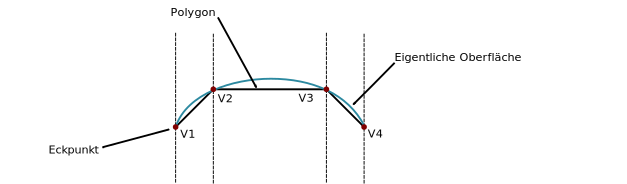
\includegraphics{img/shading_mesh.pdf}
    \caption{Illustration der Ausgangslage\protect\footnotemark}\label{
        fig:shading_mesh_illustration}
\end{figure}
\footnotetext{Eigene Darstellung mittels Inkscape, angelehnt
    an~\cite{hughes_computer_2013}}

Um einen Farbintensitätswert für einen Eckpunkt $\bm{V}_{1}$ zu berechnen, wird der
Normalenvektor des Eckpunktes (vertex normal) benötigt. Es handelt sich dabei
um den Normalenvektor der Oberfläche an der Position des Eckpunktes $\bm{V}_{1}$.

\todo[inline]{Translate/cite}
Modern shaders are really graphics programs rather than being restricted to
computing colors of points. There are geometry shaders, which can alter the
list of triangles to be processed in subsequent stages, and tessellation
shaders, which take high-level descriptions of surfaces and produce triangle
lists from them; an example is a subdivision surface shader, which might take
as input the vertices and mesh structure of a subdivision surface’s control
mesh, and produce as output a collection of tiny triangles that form a good
approximation of the limit surface. There are also vertex shaders that serve
only to transform the vertex locations, and generally have nothing to do with
eventual color.

\subsection{Flat shading --- per vertex lighting}
\label{subsec:flat_shading}

% * Calculate normal for each vertice by averaging line-segment normals, e.g.
%   (normal(V1V2) + normal(V3V4)) / 2 to determine per vertex color
%   * Image of calculated normals: line-segment (given through mesh) and vertex
% * One color per face determined by vertex' color

Bei Flat-Shading wird pro Oberfläche (Polygon) ein Eckpunkt $\bm{V}_{1}$ dieser als
farb- bzw.\ intensitätgebender Schlüsselpunkt bestimmt. Danach wird die Farbe
des Punktes als Farbe für die Oberfläche genommen.

Diese Annahme ist unter den folgenden Voraussetzungen gültig:
\begin{enumerate}
    \item{Die zugrundeliegende Lichtquelle befindet sich unendlich weit
            entfernt, so dass der Winkel zwischen dem
            Normalenvektor der Oberfläche und der Lichtquelle
            $\bm{n}\cdot{}\bm{l}$ für die gesamte Oberfläche konstant ist.}
    \item{Der Betrachter sich unendlich weit entfernt von der Oberfläche
            befindet, so dass der Winkel zwischen dem Normalenvektor der
            Oberfläche und dem Betrachter $\bm{n}\cdot{}\bm{v}$ für die
            gesamte Oberfläche konstant ist.}
    \item{Das Polygon ist eine effektive Repräsentation der Oberfläche
            und nicht nur eine Näherung einer runden Oberfläche.}
\end{enumerate}

\begin{figure}[H]
    \centering
    
\includegraphics{img/flat_shading.pdf}
    \caption{Illustration des Flat shadings\protect\footnotemark}\label{
        fig:flat_shading_illustration}
\end{figure}
\footnotetext{Eigene Darstellung mittels Inkscape, angelehnt
    an~\cite{hughes_computer_2013}}

Ist eine der ersten beiden Annahmen falsch, so muss für den Vektor der
Lichtquelle $\bm{l}$ bzw.\ den Vektor des Betrachters $\bm{v}$ ein
konstanter Wert berechnet werden.~\citet{foley_computer_1996} gibt
hier als Beispiele das Zentrum des Polygones oder den ersten Eckpunkt
des Polygones an.

\subsection{Gouraud shading --- face interpolated lighting}
\label{subsec:gouraud_shading}

Bei Gouraud-Shading handelt es sich um ein Shading-Verfahren, welches die
Farbintensitätswerte der Eckpunkte von Oberflächen eines Meshes interpoloiert.

Um den Farbintensitätswert eines Eckpunktes von Oberflächen  zu berechnen,
schlägt Gouraud die Berechnung des Durchschnittswertes der Oberflächennormalen
zweier adjazenter Liniensegmente (im 2D-Raum) bzw.\  aller adjazenter Dreiecke
(im 3D-Raum) vor.

\todo[inline]{Image explaining average calculation}

Die Berechnung des Normalenvektors eines Eckpunktes via Durchschnittswert ist
üblicherweise eine genügend gute Näherung der Oberflächennormale der
eigentlichen Oberfläche. Die Präzision hängt dabei aber klar von der
Granularität des Modelles (mesh) ab.

\subsection{Phong shading --- normal interpolated lighting}
\label{subsec:phong_shading}

\todo[inline]{Translate/cite}

Phong shading improves upon Gouraud shading and provides a better approximation
of the shading of a smooth surface. Phong shading assumes a smoothly varying
surface normal vector. The Phong interpolation method works better than Gouraud
shading when applied to a reflection model that has small specular highlights
such as the Phong reflection model.

Unlike Gouraud shading, which interpolates colors across polygons, in Phong
shading a normal vector is linearly interpolated across the surface of the
polygon from the polygon's vertex normals. The surface normal is interpolated
and normalized at each pixel and then used in a reflection model, e.g.\ the
Phong reflection model, to obtain the final pixel color. Phong shading is more
computationally expensive than Gouraud shading since the reflection model must
be computed at each pixel instead of at each vertex.
